\documentclass[class=article, crop=false, dvipdfmx, fleqn]{standalone}
\title{航空機設計法第一 \\
レポート課題3 \ 機体三面図(初期案)}
\author{学籍番号 03-170313 飯山 敬大\\
        }
\date{\today}

% packages and libraries
\usepackage[utf8]{inputenc}				%fonts
\usepackage[ipaex]{pxchfon}
\usepackage{pifont}
\usepackage{mathtools, amssymb, mathrsfs, bbm,nccmath}	%math
\usepackage{siunitx, physics}
\usepackage[table]{xcolor}				%colors
\usepackage{tabularx}
\usepackage[dvipdfmx]{graphicx}					%figures
\usepackage{subcaption, wrapfig}
\usepackage{tikz}
\usetikzlibrary{calc, patterns, decorations, angles, calendar, backgrounds, shadows, mindmap}
\usepackage{tcolorbox}					%tables
\usepackage{longtable, float, multirow, array, listliketab, enumitem, tabularx}
\usepackage{listings}					%listings
\usepackage{comment}
\usepackage{hyperref}					%URL, link
\usepackage{url}
\usepackage{pxjahyper}
\usepackage{overcite}					%setting of citation
\usepackage{pxrubrica}					%rubi
\usepackage{fancyhdr, lastpage}			%pagelayout
\usepackage{import, grffile}			%file management
\usepackage{standalone}
\usepackage{bm}
\usepackage{empheq}
\usepackage{pdfpages}
\usepackage{multicol}
% set up for siunitx
\sisetup{%
	%detect-family = true,
	detect-inline-family = math,
	detect-weight = true,
	detect-inline-weight = math,
    %input-product = *,
    quotient-mode = fraction,
	fraction-function = \frac,
	inter-unit-product = \ensuremath{\hspace{-1.5pt}\cdot\hspace{-1.5pt}},
	per-mode = symbol,
	product-units = single,
	}

% setting of line skip
\setlength{\lineskiplimit}{6pt}
\setlength{\lineskip}{6pt}

% setting of indent
\setlength{\parindent}{1zw}
\setlength{\mathindent}{5zw}

% change cite form
\renewcommand{\citeform}[1]{[#1]}

% number equations only when they are referred to in the text
\mathtoolsset{showonlyrefs=true}
%\graphicspath{{images/}{../images/}}

% set up for hyperref
\hypersetup{%
	bookmarksnumbered = true,%
	hidelinks,%
	colorlinks = true,%
	linkcolor = black,%
	urlcolor = cyan,%
	citecolor = black,%
	filecolor = magenta,%
	setpagesize = false,%
	}

\pdfstringdefDisableCommands{%
\renewcommand*{\bm}[1]{#1}%
% any other necessary redefinitions
}
% Include \subsubsection in ToC
\setcounter{tocdepth}{3}

% tabularx
\newcolumntype{C}{>{\centering\arraybackslash}X} %セル内で中央揃え
\newcolumntype{R}{>{\raggedright\arraybackslash}X} %セル内で右揃え
\newcolumntype{L}{>{\raggedleft\arraybackslash}X}

\begin{document}
\section{胴体寸法}
\subsection{胴体断面}
参考文献[2]より, 胴体は下図のようなCabin bayを5つ横に並べた形を設けることにする.1階にEconomy Class,
2階にBuisness Class とFirst Classの座席を設けることにする. 各Bayにおいて, Economy Class の座席は
通路を挟んで片側3席ずつ, Buisness Classの座席は通路を挟んで片側2席ずつとする.
一階には5つの客室用のBayを, 2階には3つの客室用Bayを設けることとする.
また高さの関係上, 荷物を客室下部に収納することはできないと考えられるので, 客室側面に荷物収納用のスペースを
設ける.  \\
シートピッチをビジネスクラス/ファーストクラス65in,エコノミークラス33[in]とし, 座席幅をエコノミークラス
21[in], ビジネスクラス30[in],通路幅をエコノミークラス25[in],ビジネスクラス30[in], 構造部材厚さを12[in]と設定する.
各bayの幅は以下のようになる.
\begin{equation}
  \begin{cases}
    \text{Economy用bay:}  \quad w_{economy} = 6 * 21 + 25 = 151 [in] \\
    \text{Buisness用bay:} \quad w_{buisness} = 4 * 30 + 30 = 150 [in]
  \end{cases}
\end{equation}
これで1階と2階のBayの幅はほぼ同じになる. 各bayを区切る壁の厚さを$w_{wall} = 5[in]$とすると, 胴体内径(幅)と外径(幅)は最も広くなる場所で,
\begin{align}
   D_{in} &= w_{economy} * 5 + w_{wall} * 4 \\
          &= 151 \times 5 + 5 \times 4 =775 [in]\\
   D_{out} &= D_{in} + 12 = 787[in] \approx 65.5[ft]
\end{align}
となる. \\
以上より, 客室の断面は下図のように表せる.
\begin{figure}[H]
  \begin{center}
  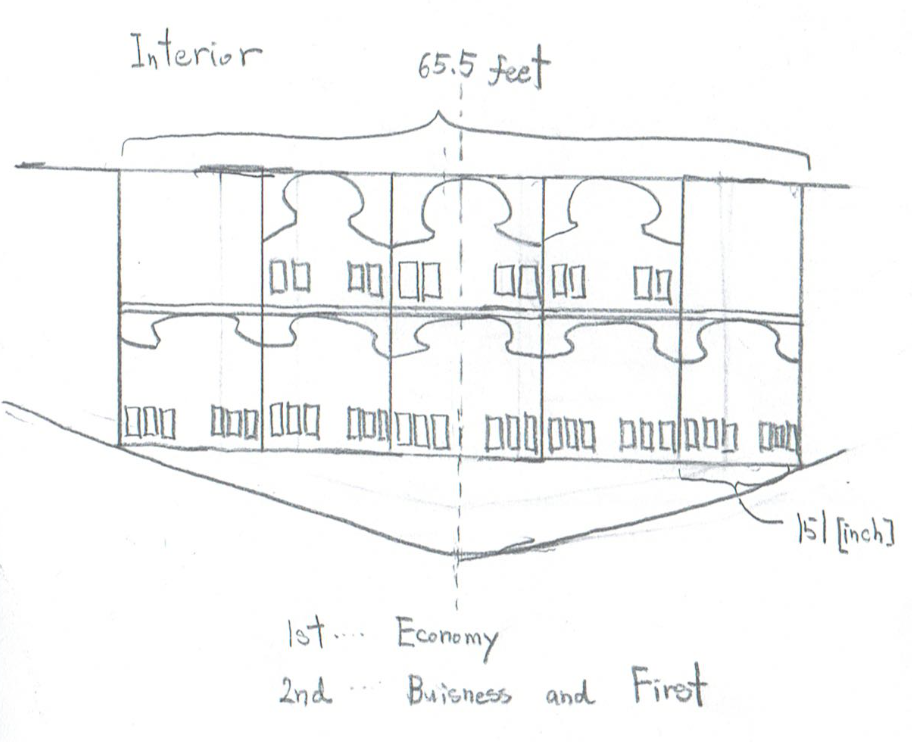
\includegraphics[width=8cm]{../images/frontview.png}
  \caption{客室正面図(寸法は考慮していない)}
  \label{fig::frontview}
\end{center}
\end{figure}

\begin{figure}[H]
  \begin{center}
  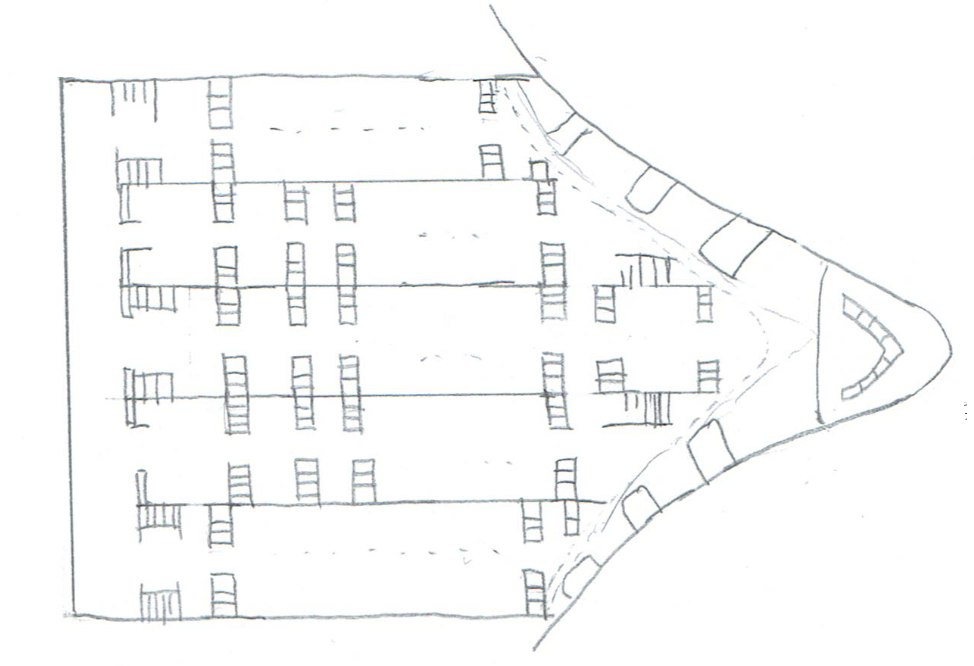
\includegraphics[width=8cm]{../images/overview.png}
  \caption{客室上面図(寸法は考慮していない)}
  \label{fig::overview}
\end{center}
\end{figure}


\subsection{客室長さ}
ファーストクラス + ビジネスクラス64名, エコノミークラス354名とすれば, 一列あたりの人数は
ビジネス・ファーストクラスは$4 \times 3 = 12$名, エコノミークラスは$6 \times 5 = 30$名
であるから, 必要な列数はビジネス・ファーストクラスが$ 64/12 = 6$列,
エコノミークラスは$354/30 = 12$ 列であるから, それぞれのbayの長さは,前後に
\begin{equation}
  \hspace{-10mm}
  \begin{cases}
  \text{Economy用bay:}  \quad l_{economy} = 6 \times 65[in] + 2 \times 25[in] = 37.1 [ft] \\
  \text{Buisness用bay:} \quad l_{buisness} = 12 \times 33[in] + 2 \times 25[in] = 36.6 [ft]
\end{cases}
\end{equation}
となり大体等しくなるので, 整合性が取れる.
また客室の前後に廊下やトイレ, 階段等の設備を備えることを踏まえて, 客室長さ(各Bayの長さ)を,
\begin{equation}
  l_c = 45[ft]
\end{equation}
とする.

\subsection{客室高さについての検討}
最後に,2階分の高さを確保することができるか検討する.
第3章で示した図のように, 胴体全長を翼根部で100[ft]とする.

すると, 各部分でのコード長と主翼厚さの概形は下のグラフのようになる.(実際は
滑らかに変化する)
\begin{figure}[H]
  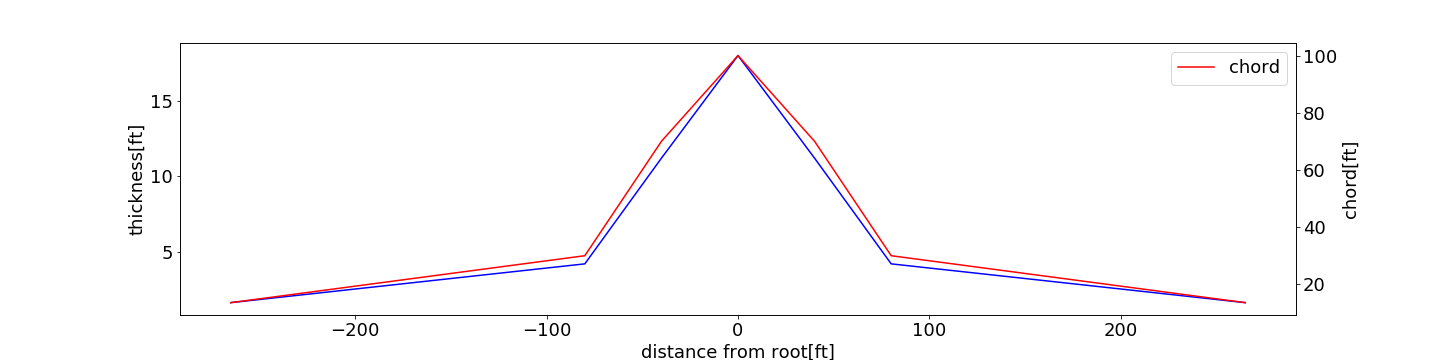
\includegraphics[width=12cm]{../images/wingthickness.png}
  \caption{最大厚さとコード長}
  \label{fig::thickness}
\end{figure}
胴体の幅が65.5feetであるから, 胴体の最も外側の部分の主翼の最大厚さが12.2[ft],コード長は
74[ft]であるから, 2階の両端のBayには客室は配置されない(荷物を収納する場所とする)ことも
考慮に入れると, 十分に2階立ての客室(全長45[ft])を収容できると考えられる.

\end{document}
